\subsection{Formulazione debole dell'equazione di Poisson (FEM)}
\begin{equation*}
\begin{cases}
\nabla^2u = f & \text{in }\Omega\\
\left. u \right|_{\partial\Omega} = g
\end{cases}
\end{equation*}
$$
u \in C^2(\Omega),\ f \in C^0(\Omega),\ g\in C^0(\partial\Omega)
$$
In queste condizione la soluzione esiste ed è unica.
La soluzione di classe $C^2$ viene chiamata \textbf{forte} in termini di regolarità
ossia è molto regolare.

Normalmente quando si applica il \textit{metodo degli elementi finiti} (FEM) 
i requisiti sulla funzione incognita $u$ sono meno stringenti e si
parla di soluzione \textbf{debole}.

Si considera uno spazio di funzioni \textit{test} chiamate funzioni
``peso''  $p \in C^1_0\ : \ p(\partial\Omega) = 0$

Moltiplicando ambi i membri dell'equazione di Poisson e integrando si ottiene:
$$
\iiint_\Omega p\nabla^2 u dV = \iiint_\Omega p f dV
$$
Ricordando l'identità vettoriale $p\nabla^2 u = \nabla\cdot \left(p\nabla u\right) - \nabla p\cdot \nabla u $

Sostituendo si ottiene:
$$
\iiint_\Omega p f dV = \iiint_{\Omega} \left(\nabla\cdot\left(p\nabla u\right)-\nabla p\cdot\nabla u\right)dV
$$
Applicando il teorema della divergenza
$$
\iiint_\Omega p f dV = \cancel{\iint_{\partial\Omega} p \frac{\partial u}{\partial n}dS} - \iiint_\Omega \nabla p\cdot\nabla u\ dV
$$
Siccome la funzione $p$ test scelta è nulla sulla frontiera, il primo termine della differenza si azzera:
$$
\iiint_\Omega p f dV = \iiint_\Omega -\nabla p\cdot\nabla u\ dV\ \ \forall\ p\in C^1_0(\Omega)
$$
Quella appena ottenuta è proprio la formazione debole del BVP iniziale.

Introducendo $u_\partial : u_\partial = g\ \text{su } \partial\Omega\ : \ u = \hat{u} + u_\partial$ ossia prolungando
la funzione $g$ all'interno del dominio, si può ricavare la funzione $\hat{u}$ differenza tra le due.

Si vede dunque che $\hat{u}$ è soluzione di un BVP per la stessa equazioni con condizioni di
Dirichlet omogenee, ossia $\hat{u} = 0\ \text{su } \partial\Omega$.

Sostituendo la funzione $u$ estesa nell'integrale precedente si ottiene
$$
-\iiint_\Omega \nabla p \cdot \nabla\hat{u}\  dV = \iiint_\Omega p f dV +
\iiint_\Omega \nabla p \cdot \nabla u_\partial\ dV\ \forall\ p\in C^1_0(\Omega)
$$
I due integrali a destra dell'uguaglianza sono termini noti, l'espressione rappresenta
una famiglia di equazioni integrali nell'incognita $\hat{u}$ al variare
di $p$ nello spazio delle funzioni test.

\newpage
\subparagraph{\href{https://it.wikipedia.org/wiki/Metodo_di_Gal\%C3\%ABrkin}{Metodo di Galërkin}}
Consiste nel ricercare una soluzione espressa mediante la base di uno spazio
a dimensione finita chiamato ad esempio $W^0_M$ dove $M$ è il numero di
gradi di libertà da utilizzare ossia quanto più accurata sarà la soluzione,
se al limite $M$ fosse infinito avrei una soluzione identica al continuo.

Supposta una base $\hat{u}_M$ per questo spazio di funzioni che si 
annullano sulla frontiera a dimensione finita $M$
$$
\hat{u}_M = \sum_{k = 1}^{M} a_k w_k \ \ \text{ con } w_k \text{ funzioni di base di } W_m^0
$$
Sostituendo nell'integrale del paragrafo precedente
$$
-\iiint_\Omega \nabla w_h \cdot \nabla \left(\sum_{k=1}^{M} a_k w_k \right) dV = 
\iiint_\Omega w_h f dV + \iiint_\Omega \nabla w_h \cdot \nabla u_\partial\ dV\ \ h=1,...,M
$$
I coefficienti $a_k$ per linearità si possono tirar fuori dall'integrale
$$
-\sum_{k=1}^M \left(\iiint_\Omega \nabla w_h \cdot \nabla w_k\ dV \right) a_k = 
\iiint_\Omega w_h f dV + \iiint_\Omega \nabla w_h \cdot \nabla u_\partial\ dV
$$
Svolgendo l'integrale tra parentesi e risolvendo gli integrali a destra
$$
-\sum_{k=1}^M L_{hk} a_k = b_h\ \ h=1,...,M
$$
L'equazione ottenuta si trasforma in un sistema lineare algebrico del tipo:
$$
\underline{L}_M \cdot \underline{a}_M = \underline{b}_M
$$
Se si ipotizza una forma per le funzioni test è possibile calcolare i coefficienti
$L_{hk}$ e risolvere il sistema.

\newpage
\subparagraph{Metodo degli elementi finiti}
\begin{figure}[H]
\centering
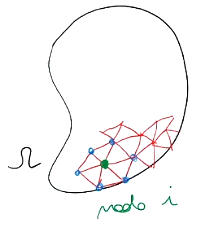
\includegraphics[width = 0.2\linewidth]{esempio_dominio_mesh}
\caption{Esempio dominio con MESH}
\end{figure}
Consiste nel partizionare ad esempio con strutture triangolari o tetraediche un dominio.
Si definisce su ogni nodo $i$ della griglia una funzione test $w_i$

$$
w_i(\underline{x}) = \begin{cases}
1 & \text{se } \underline{x} = \underline{x}_i\\
0 & \text{se } \underline{x} \neq \underline{x}_i\\
&\text{lineare intorno al nodo }\underline{x}_i
\end{cases}
$$
Vengono definite funzioni ``a tenda'' data la loro somiglianza ad una tenda canadese.
È possibile calcolare tutti i coefficienti una volta ottenuta la \textit{MESH} del
dominio, ossia la sua completa triangolazione.
Una volta nota è possibile assegnare facilmente le funzioni tenda e calcolare i
coefficienti $L_{hk}$ e $b_h$ note le funzioni $f$ e $g$.
All'aumentare di $M$ ossia del numero di nodi migliora la descrizione
della geometria.

In MATLAB è possibile usare la \textit{Partial Differential Equation Toolbox}, per 
gli amici ``pdetool'' per accedere ad un'interfaccia grafica che permette
di impostare una geometria e risolvere questo genere di problemi.
